This pipeline transforms raw data from the Sensible DTU experiment into ordered, clean, datamatrices of behavioral indicators, personality traits and personality archetype distances for each participant, labeled $\matr{X}$, $\matr{Y}$ and $\matr{D}$ respectively. It is constructed using principles from software engineering such as reusability and version control. The pipeline is implemented as a set of smaller modules that each execute a task. All modules rely on the virtual IPython Notebook environment made available to researchers associated with the Social Fabric project (see Sec. \ref{subsec:sensibleDTU}). The pipeline is designed to allow the researcher to extract data for specific date ranges and with hour-of-day- and day-of-week- restrictions. It relies on a modified verision of the Python module \textit{bandicoot} for computing behavioral indicators. 

Consider Fig. \ref{fig:preprocessing_pipeline} as a reference for the following introduction to the pipeline. The researcher first enters the \texttt{create\_user\_records} IPython notebook to create data records for each user in a desired time range using the \texttt{load\_sensible\_data} module. When data is loaded for a new time range, \texttt{load\_sensible\_data} caches the raw data to save time and API load in case of future uses, then looks for timezone and location references for each user which, if not found, are automatically created. The module then returns semi-raw datasets for each datatype (\texttt{text}, \texttt{call}, \texttt{F2F}, \texttt{stop}, \texttt{screen}) where timestamps are corrected according to timezone and DST, and where a location label ('home', 'campus', 'dorm', 'friday\_bar' or 'other') is added to \texttt{stop}-records using a \textit{point-inside-polygon} algorithm\mcite{pointInsidePolygon}. Each semi-raw dataset is split into seperate datasets for each user, and stored. Using the \texttt{create\_datasets} IPython Notebook which relies on the bandicoot library to compute behavioral indicators for each user constructing a datamatrix $\matr{X}$ which has a row for each user and a column for each indicator. For each user the corresponding Big Five personality traits are computed using the \texttt{load\_big\_five\_data} module. Furthermore distances from precomputed archetypes are computed using the \texttt{compute\_thetas} module.

\begin{figure}
	\centering
	\begin{minipage}[l]{0.80\textwidth}
		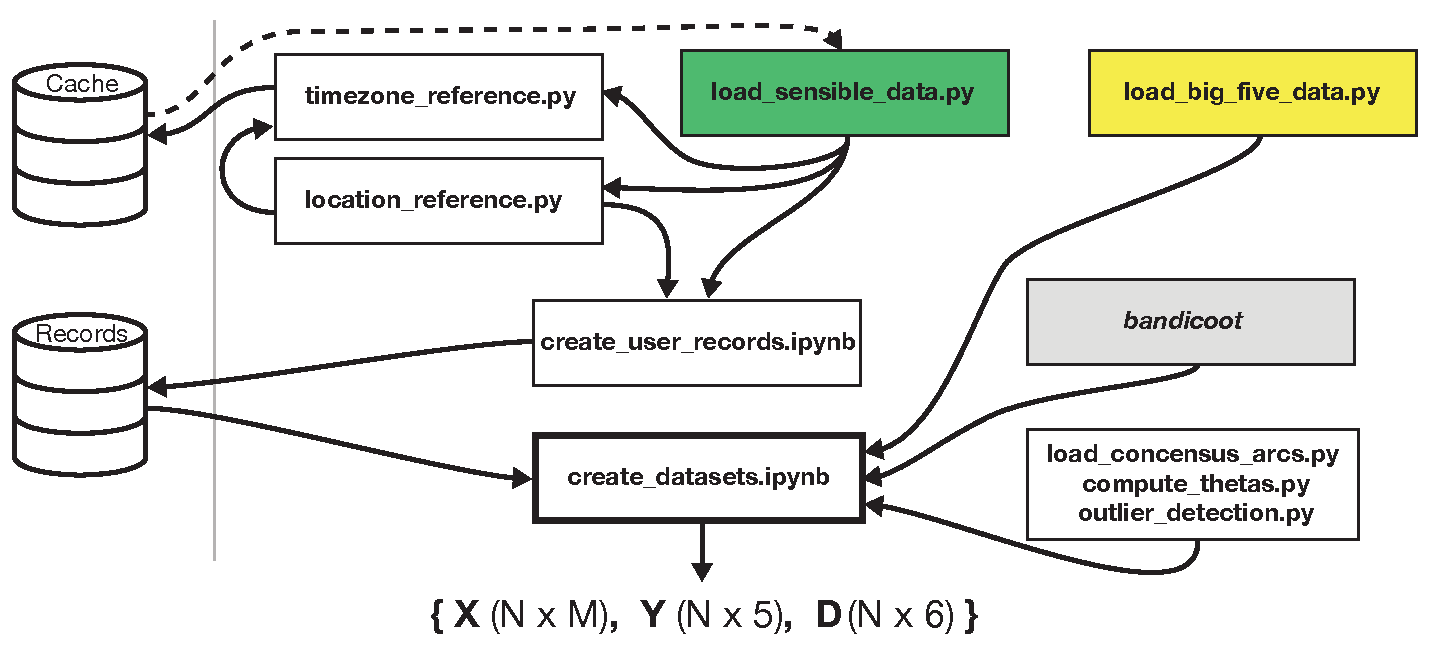
\includegraphics[width=\linewidth]{figures/preprocessing_pipeline}
	\end{minipage}
	\begin{minipage}[r]{0.19\textwidth}
		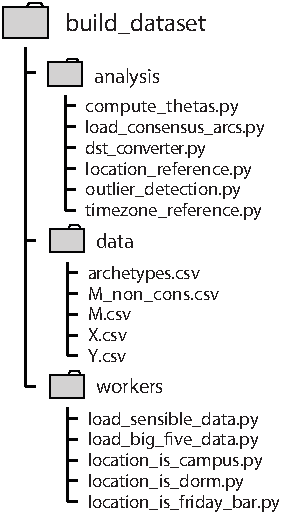
\includegraphics[width=\linewidth]{figures/preprocessing_repo}
	\end{minipage}
	\caption{\label{fig:preprocessing_pipeline}Preprocessing pipeline implemented on the virtual IPython notebook environment (see Sec. \ref{subsec:sensibleDTU}). The researcher first creates records for all users in a format that is accepted by the modified version of bandicoot, then uses bandicoot and pipeline submodules to compute three datamatrices: behavioral indicators $\matr{X}$, Big Five personality traits $\matr{Y}$ and weighted euclidian distances from precomputed consensus archetypes $\matr{D}$.}.
\end{figure}

The analysis pipeline is made available on Github at:\\

\url{https://github.com/ulfaslak/MScProject-build-dataset}